It begins! Today I'll be at the Doctoral Consortium (DC) -- my goal with the notes is both to give folks a sense of what a DC entails, and to share the exciting research of some great grad students.

\subsection{Overview of the DC}

%\dnote{todo.}
I {\it highly} recommend doing a doctoral consortium at some point during grad school. I learned a huge amount from the experience --

For those that don't know, a DC involves preparing a short abstract summarizing your work, and giving a 10-20 minute presentation to your peers and their montors. Each student participating is assigned a mentor (from their area) that helps with preparing your presentation and gives you more general advice on your research. \\

It was a great experience! I had the pleasure of meeting many wonderful grad students and hearing about the diversity of exciting work and learning from their methods and ideas.



\subsection{Neeti Pokhriyal: Multi-View Learning From Disparate Sources for Poverty Mapping}

{\bf Focus:} Learning from multiple disparate data sources, applied to sustainability and biometrics. \\

Specific Application: Povert mapping. Spatial representation of economic deprivations for a country. A major tool for policy planners. \\

Current method is a household survey, which is 1) costly, 2) time consuming, 3) only available for small samples. \\

{\bf Research Goal:} Get accurate, spatially detailed and diagnostic poverty maps for a country. \\

Lots of data available via weather, street maps, economic data, mobile phones, satellite imagery. But! Each of these data sources are structured very different. \\

\begin{figure}[h!]
    \centering
    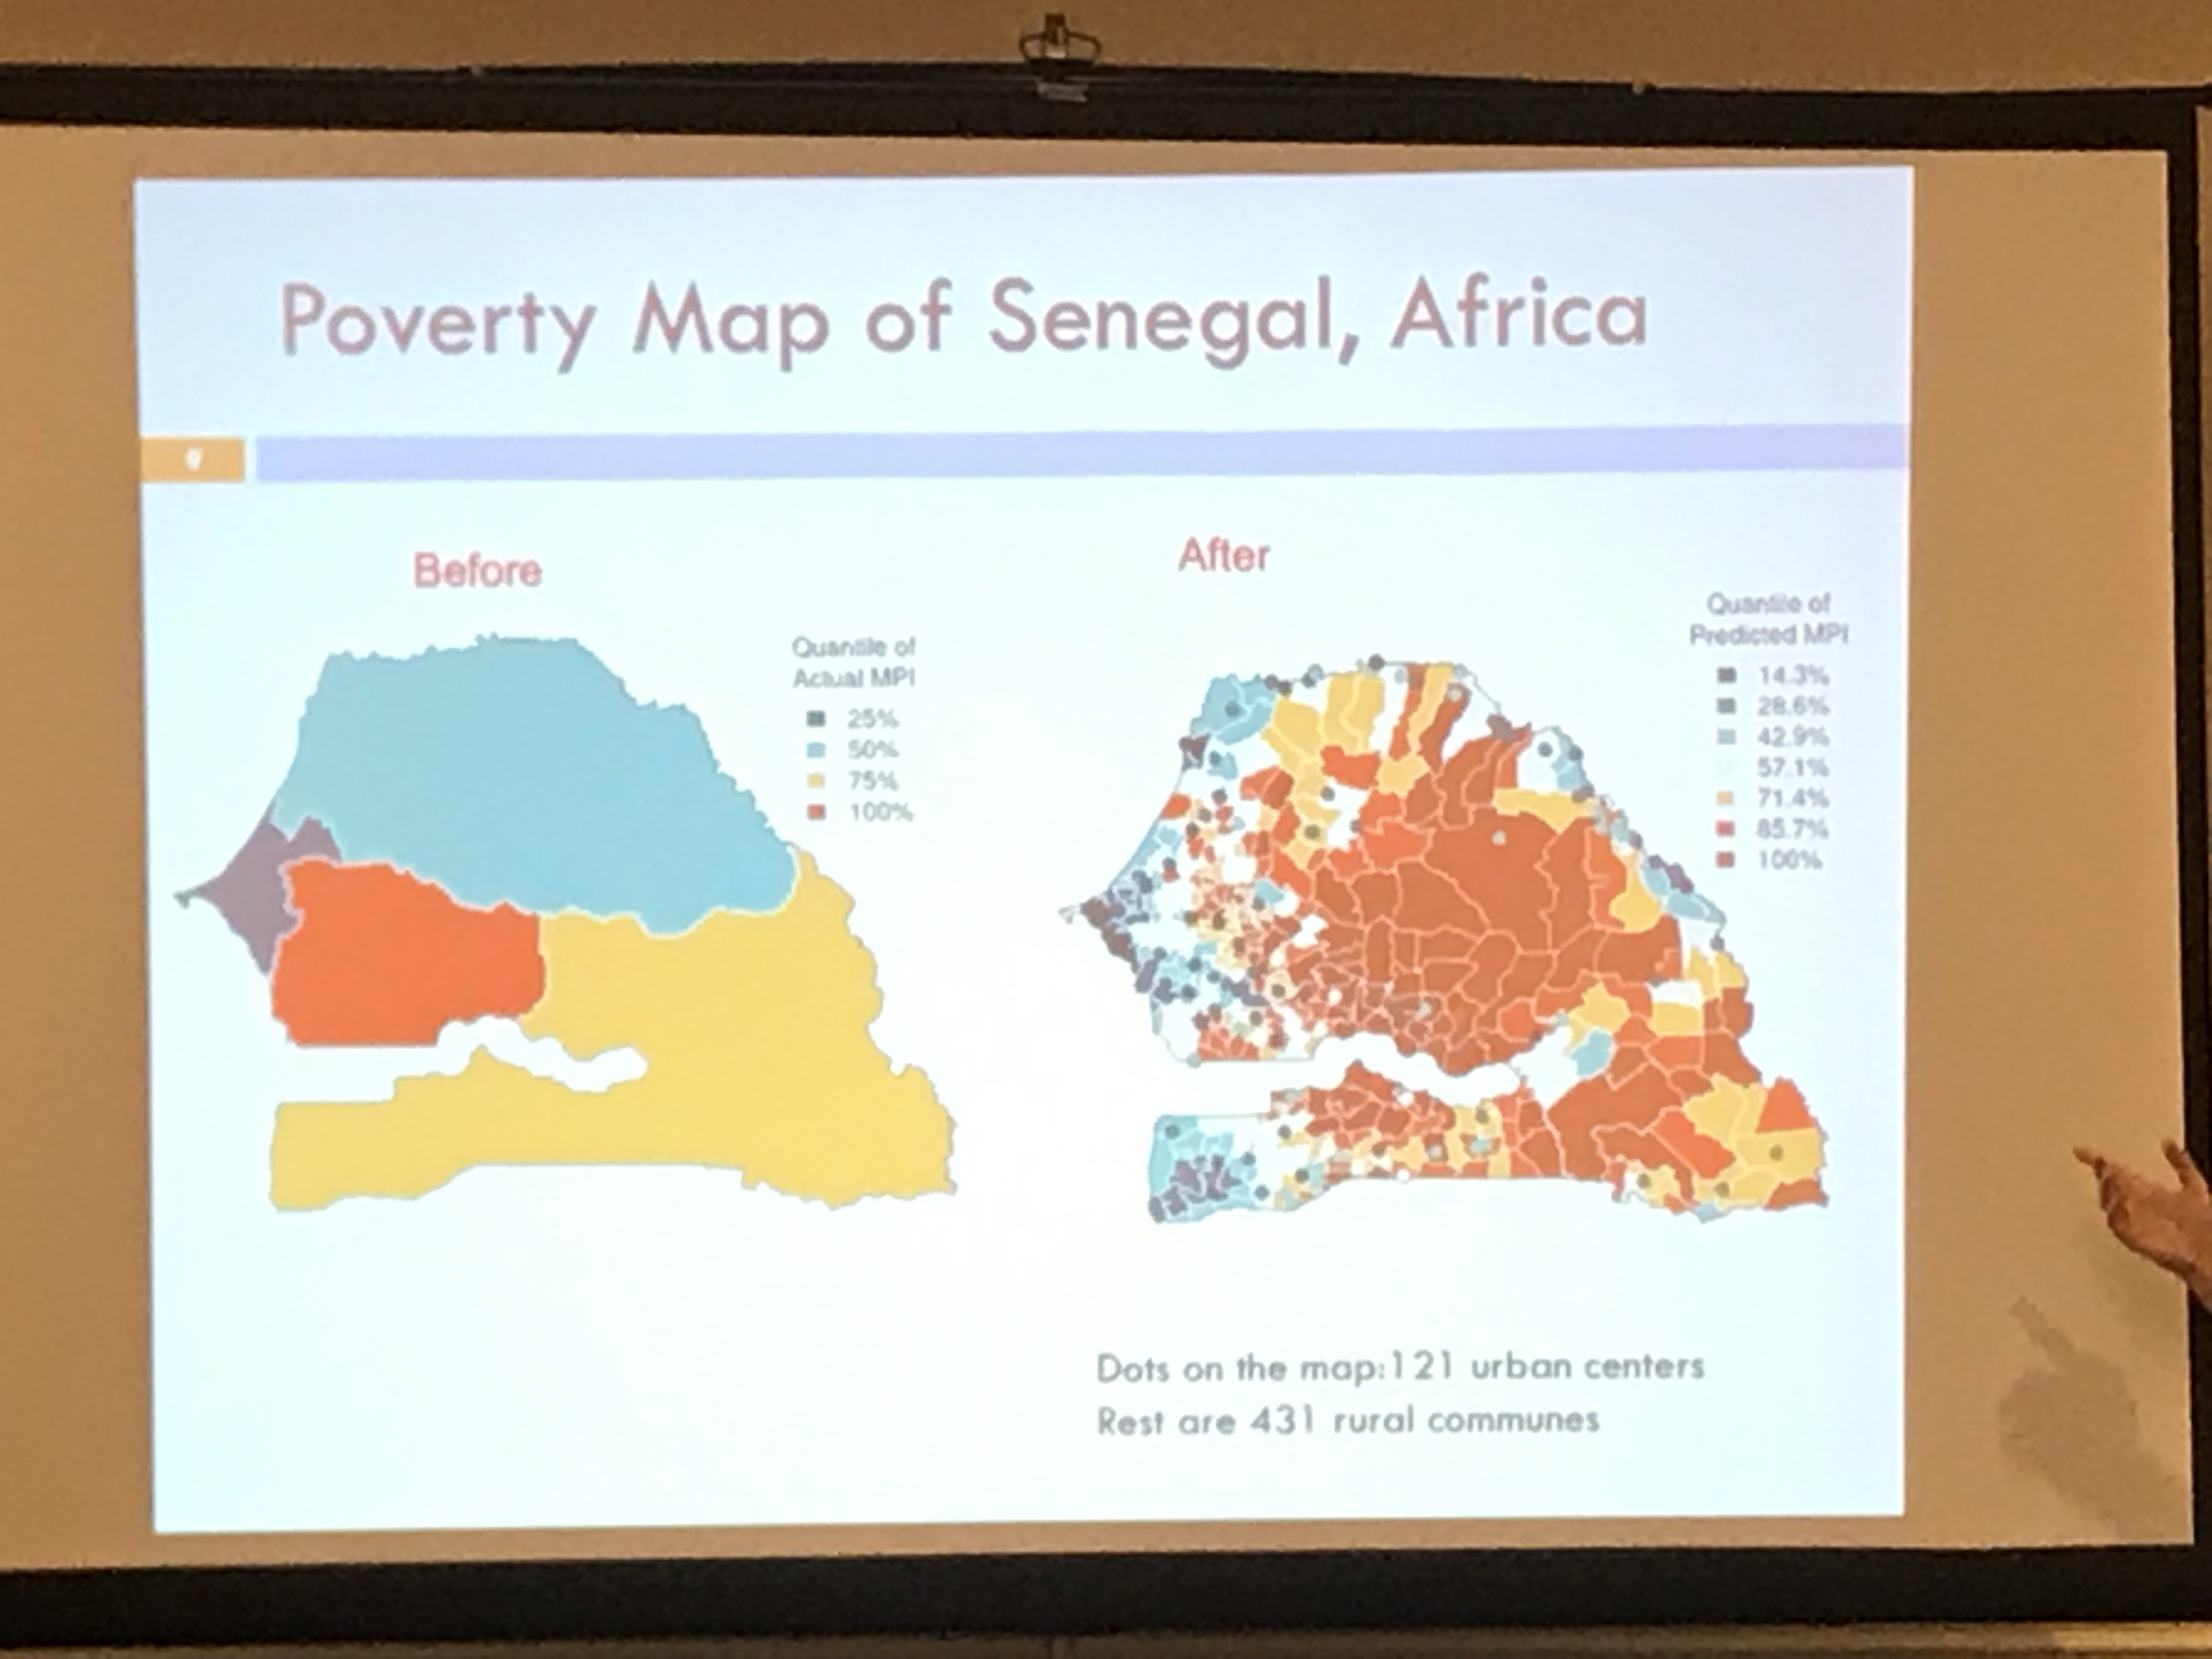
\includegraphics[width=0.5\textwidth]{images/pov_map.JPG}
    \caption{Higher fidelity poverty prediction}
    \label{fig:pov_map}
\end{figure}

\ddef{Multi-View Learning}{A style of learning takes as input separate, semantically distinct kinds of data, and brings them together into a factorized representation for use in predictive models.}

Method: learn a Gaussian Process (GP) Regression model combined with elastic net regulariation~\cite{zou2005regularization}. \\

Using this model yields the map pictured in Figure~\ref{fig:pov_map}. Then perform quantitive analysis and validates that their model is making high quality predictions by comparing to census data. \\

{\bf Objective 2:} learn a factorized representation from multiple data sources. The hope is that we can disentangle explanatory factors that are unique to each data source. \\

Sort of an EM like approach:
\begin{enumerate}
    \item {\it Learning Step:} MAp views $Y$ and $Z$ to shared subspaces $X_i, \ldots$.
    \item {\it Inference Step:} Perform inference on these subspaces.
\end{enumerate}

Q: Main question, then: how do we learn the shared subspace?\\

A: Separate data belonging to different class across different views is maximized, while ensuring alignment of projects from each view to the shared space. Can be solved using a Generalized Eigenvalue problem, or using the kernel trick.



\spacerule
\subsection{Negar Hassanpour: Counterfactual Reasoning for Causal Effect Estimation}

{\bf Problem:} Consider Mr. Smith, who has a disease and some known properties (age, BMI, etc.). Doctor provides treatment X and observes the effect of treatment X (but does {\it not} get data about the counterfactul: what would have happened if doc had applied treatment Y?). \\

{\bf Goal:} Estimate the ``Individual Treatment Effects" (ITE) -- how does treatment X compare to Y? \\

Datasets:
\begin{itemize}
    \item Randomized Controlled Trial (RCT): See lots of both X and Y. But, it's expensive (lots of trials) and unethical (giving placebos when you know the right treatment).
    \item Observational Study: provide the preferred treatment. But, sample selection bias.
    
    {\it Example:} Treating heart disease, a doc prescribes surgery to younger patients and medication to older patients. Compare survival time -- but, clear bias in who gets what treatment.
\end{itemize}

This is a really fundamental problem called ``sample selection bias" -- rich patients receiving expensive treatment vs. poor patients receiving cheap treatment and so on. \\

Overview of this work:
\begin{itemize}
    \item Generate realistic synthetic datasets for evaluating these methods (since good data is hard to come by)
    
    $\ra$ Take an RCT and augment it with synthetic data.
    
    \item Use representation learning to reduce sample selection bias.
    
    $\ra$ Want $Pr(\phi(x) \mid t=0) \approx Pr(\phi(x) \mid t=1)$ to be similar, with $\phi$ the learned representation and $t$ the treatment.
    
    \item Learn underlying causal mechanism with generative models.
    
    $\ra$ Learn causal relationships between treatments and outcomes by using generative models. Can we identify the latent sources of outcome from observational dataset?
    
    \item Perform survival predictions.
    
    $\ra$ Can we predict outcomes that are censored or take place after studies end?
    
    \item Going beyond binary treatments
    
    $\ra$ Many, but not all, treatments are binary. Can we go beyond this to categorical or real valued treatments?
    
    \item Providing a course of treatment
    
    $\ra$ Call on reinforcement learning.

\end{itemize}



\spacerule
\subsection{Khimya Khetarpal: Learning Temporal Abstraction Across Action \& Perception}

Q: How should an AI agent efficiently represent, learn, and use knowledge of the world? \\

A: Let's use temporal abstractions! \\

Example: preparing breakfast. Lots of subtasks/activities involved like (high level): choose eggs, type of toast (mid level) chop vegetables, get butter, and (low level) wrist and arm movements. \\

\ddef{Options~\cite{sutton1999between}}{An option formalizes a skill/temporally extended action as a triple: $\langle, I, \beta, \pi \rangle$, where $I \subseteq S$ is a initiation set, $\beta : S \ra \Pr(S)$ is a termination probability, and $\pi : S \ra A$ is a policy.}

Example: A robot navigates through a house between two rooms. To do so, it has to open a door. We let $I$ denote the states where the door is closed, $\beta$ is 1 when the door is open and 0 otherwise, and $\pi$ opens the door. Then, this option defines the ``open the door" skill. \\

{\bf Main Question}: Can we learn useful temporal abstractions? \\

{\bf Hypothesis:} Learning options which are specialized in situations of specific interest can be used to get the right temporal abstractions. \\

Motivation: AI agents should be able to learn and develop skills continually, hierarchically, and incrementally over time. \\

So, imagine we had a house decomposed into different rooms. Then we would like to learn skills that take the agent between each room. Further, the agent should be able to transfer for one agent to another. \\

{\bf Objective 1:} Learn options and interest functions simultaneously. \\

New idea: break the option-critic assumption~\cite{bacon2017option} that $I = S$. Instead, consider an interest function:
\ddef{Interest Function}{An interest function is an indication of the extent to which an option is interested in state $s$.}

Now learn a policy over options and an interest function -- we can jointly optimized over both things. Derive the policy gradient theorem for interest functions, intra-option policy, and the termination function. \\

\begin{figure}[h!]
    \centering
    \includegraphics[width=0.5\textwidth]{images/four_room.png}
    \caption{Learned interest functions}
    \label{fig:opt_four}
\end{figure}

Also explore learning interest functions in continuous control tasks, showing nice separation between the learn options. \\

{\bf Objective 2:} Consider a never-ending stream of perceptual data. We'd like to learn a stream of percepts and behavior over time. \\

Challenges:
\begin{itemize}
    \item How can we the agent automatically learn features which are meaningful pseudo rewards?
    \item Where to task descriptions come from?
    \item How can we achieve the most general options without hand designing tasks/rewards?
    \item Evaluation in a lifelong learning task? Benchmarks?
\end{itemize}


\spacerule
\subsection{Ana Valeria Gonzalez-Garduño: RL for Low Resource Dialogue Systems}

{\bf Goal 1:} Create more informed approaches to dialogue generation. \\

{\bf Goal 2:} Use RL for domain adaption in goal oriented dialogue. \\

(And: can we do this in a language agnostic way? So, introduce models that can work with any/many languages). \\

Dialogue systems are divided into two subfields:
\begin{enumerate}
    \item {\it Open ended dialogue generation:} typically use encoder-decoder architectures
    \item {\it Goal oriented dialogue:} predominantly tackle using ``pipeline" methods. So, automatic speech recognition unit, then an understanding unit, and so on.
\end{enumerate}

Current Focus: ``state tracking". That is, state tracking deals with inferring the user intent or belief state during the conversation. \\

But, limitation: intents usually rely on a particular ontology that defines which intents are valid. \\

Current Status of the Project: Bridge the gap inb goal oriented dialogue. Main goal: can we get rid of the need for annotations? \\

General idea: given a bot's utterance (``how can I help?"), and a user response (``I want to change payment methods"), we want to find a relevant query from prior conversations to identify what the user said. Or really, use it to condition the decoder. \\

Result: this model works very well! On BLEU their model performs favorably, but more importantly, on a human evaluation, their responses were consistently chosen over the baseline. \\

Q: But, what if our domain is not in the pool of relevant conversations? \\

A: Work in progress! Idea $\ra$ Use RL:
\begin{enumerate}
    \item Phase 1: Use existing data for state tracking, pretrain models in a supervised manner.
    
    $\ra$ Turn level supervision, slots and values represented using word embeddings.
    
    \item Phase 2: Use RL to finetune pretrained model.
    
    $\ra$ Rely on dialogue level supervision (joint goal accuracy) as reward. So, how many slot-values (``Food-Mexican, Price-Cheap"), to determine the reward.
\end{enumerate}

Challenges in using RL for state tracking: dialogue is long (credit assignment is hard!), sample efficiency, might be able to leverage curriculum learning. \\

Main Future Direction: Enable dialogue state transition model to generate new unseen slots.


\spacerule
\subsection{AAAI Tutorial: Eugene Freuder on How to Give a Talk}


Start with an example! Or a counter example. \\

These are just his conclusions! So decide for yourself, of course. \\

This talk is not intended to be mean spirited -- he'll be talking about mistakes people make. \\

Meta-message: presenting a talk is a skill that can be studied and practiced! And it's worth doing -- spend years researching and 10 minutes presenting. The 10 minutes should be polished. \\

Six Points:
\begin{enumerate}
    \item Convey Enthusiasm
    \item Make it Easy to follow
    \item Employ examples
    \item Expressive
    \item Enhance your presentation with visuals/dynamic material
    \item Engage the audience
\end{enumerate}


\subsubsection{Enthusiasm}
The secret of a good talk: {\bf Enthusiasm!}\\

$\ra$ If you're not enthusiastic about your work, how do you expect anyone else to be? \\

Fear of public speaking: ``glausophobia" -- ranked as the most common fear in the USA (more so than spiders/death). \\

Q: How do you get over this fear? \\

A: Remember the audience is on your side! Breathe. Drink water. \\

Tricks:
\begin{itemize}
    \item Look over their heads (instead of in their faces-- can be easier).
    \item Or, turn it into an individual conversation, or a bunch of individual conversations.
    \item Science is fun! So have fun.
\end{itemize} 

Sometimes it feels like there's the me giving the talk and the me monitoring me giving the talk. Unfortunate, potentially, as I'm then not present.\\

It is {\bf really} hard to be too enthusiastic. The speaker is standing on a chair to demonstrate enthusiasm --\\


\subsubsection{Easy to Follow}

One major goal of the talk: get people to read and build on your work. Details are in the paper-- job in the talk is to get them to read the paper. \\

KISS principle: Keep It Simple Stupid! \\

Story from Feynman's lost lecture: someone asked Feynman to prepare a lecture on some complicated physics concept related to particle spin. Feynman said he would go off and work on it for a few days and come back and give a lecture: ``I'll be able to give a freshmen level lecture in a few days!". But then he came back: ``Okay, I couldn't do it. I couldn't turn it into a freshmen level lecture. {\it Which means we don't yet understand it yet}." \\

Audience doesn't distinguish hard work from the researcher having a hard time explaining it. \\

Let them see the forest -- not the trees. \\

Explain math/formalisms with visuals and metaphor. Minimize definitions, don't overestimate audience. \\

People make talks too difficult by going through material too quickly, or trying to force too much in. Time yourself!

\subsubsection{Use Examples}

Start with an example! Even before the title/introduction. \dnote{Hm! Bold move. Hard to do this in a conference, to me. But it's a neat idea.} \\

He played a clip from a TED talk (Niri G?) where the speaker opened just with ``Two twin domes...". It was engaging. \\

Even if you don't start with one -- use one. It can be hard to make the example simple enough. \\

Make your example(s):
\begin{itemize}
    \item Illustrate what you've done
    \item Simple
    \item Concrete
    \item Only add complexity later (or use a running example!)
\end{itemize}

\subsubsection{Be Expressive}

Use your voice and body language to be expressive. \\

Do's and Dont's:
\begin{itemize}
    \item[{\bf Do:}]  smile (he played Nat King Cole!), listen to yourself beforehand (and look for ``ums", body swaying, etc), try to make it a conversation (not a declamation), vary your voice (louder/softer, higher/lower), pause occasionally, articulate, look people in the eye, turn off your phone, silence computer.
    
    \vspace{4mm}
    
    \item[{\bf Don't:}] Read from a prompt, speak in a monotone, speak too fast or too slow, be distracting (like playing with your hair, rocking back and forth or front to back $\ra$ a good alternative is to hang onto the lectern), say ``um"/``uh" too much, mumble, fidget, turn around a face the screen, look at your laptop too much.
\end{itemize}

\subsubsection{Enhance your talk with visuals/dynamics}

Do's and Dont's:
\begin{itemize}
    \item[{\bf Do:}] use visuals, minimize text, keep notes for yourself, remember short term memory of audience (repeat details, highlight big things, etc.), pull out what is important. 
    \vspace{4mm}
    
    \item[{\bf Don't:}] use bulleted lists.
\end{itemize}

\subsubsection{Engage the Audience}

Q: How do you engage an audience directly? \\

A: Ask questions! \\

Consider why your audience is here: they want to hear what you did. Tell them right away what you're going to do. Big results at the beginning. \\

Can turn your talk into a story:
\begin{itemize}
    \item A problem to be solved. Someone came to me in a company with a problem, and so on.
    \item Could be the ``2x2 matrix" story: folks have done Red things and Blue things, and folks have done Small things and Big things, but no one has done Big Red things! I'm going to do that.
    \item Could contradict conventional wisdom
    \item The ``journey" and not just the endpoint.
\end{itemize}

Make your talk fun! ``A spoonful of sugar makes the medicine go down." Use gimmicks, like: playing songs, use props, video, etc. \\

Hypothesis: on average, at a CS conference, by the time you reach the halfway point, at least half the people would be tuned out. \\

$\ra$ So: if the hypothesis is even close to being right, think of the waste! \\

\spacerule
\subsection{Aida Rahmattalabi: Robust Peer-Monitoring on Graphs}

{\bf Problem:} Suicide is a critical public health problem in the US. Second leading cause of death among students. \\

One approach: gatekeeper training (suicide prevention program). Can identify warning signs, but can only train limited number of individuals. \\

{\bf Main Goal:} Improve gate keeper training with social network information by taking into account characteristics of individals in the population. \\

Technical problem: optimize:
\begin{equation}
    \max_{x,y} \sum_{n \in N} y_n,
\end{equation}
subject to $x \in \mc{X}$ and $y \in \mc{Y}$, which define the feasible sets of possible choices of trainers. \\

Basically: social characteristics are very important in assigning a gatekeeper. So, impose constraints on who is chosen as a gatekepeer (based on things like race/gender). \\

But, new problem: participation uncertainty. Not all chosen trainers might not participate. \\

Optimization problem is formulated as:
\begin{equation}
    \max_{x \in \mc{X}} \min_{\eps \in E} \sum_{n \in N} y_n(x,\eps),
\end{equation}
where the $x$ is the gatekeeper we choose, and natre is acting adversarially over choice of $\sigma$ which determines participation rate. $y_n(x,\epc)$ denotes the coverage for each of the $n$ individuals. Can cast this as a polynomial size mixed integer program which is nice and tractable. That is, main result:
\begin{theorem}
For a fixed vale of $K$, their main optimization problem (the ``$k$ adaptibility problem"), can be reformulated exactly as a polynomially sized mixed integer linear program.
\end{theorem}

Experiments: compare to a greedy robust approach on a real social network. Measuring ``coverage", which is captured by the function $y$ above. Also evaluate according to a ``Price of Fairness".

\spacerule
\subsection{Nikhil Bhargava	: Multi-Agent Coordination under Uncertain Communication}

Consider under water gliders: they go underwater for months at a time, so we can't actually communicate with them very often.\\

So, most folks usually use a ``real time executive" (RTE), which is a centralized, real-time means of dispatching actions to different agents. \\

But: in reality, too much uncertainy in action execution. So, RTEs often include state updates based on the outcome of action executions. \\

Lots of prior work on RTEs that can handle highly expressive plans, can adapt to uncertainty, etc. \\

But back to our gliders: lots of different autonomous agents with uncertainty in actions and communications. \\

{\bf Goal:} Can we upgrade this notion of an RTE into a multi-agent system? \\

Three core ideas/changes to the traditional RTE model:
\begin{enumerate}
    \item Multi-agent aware planning
    
    $\ra$ Turn Simple Temporal Networks With Uncertainty (STNUs) into DTNUs/POSTNUs, which is analogous to turning MDPs into DecPOMDPs, POMDPs.
    
    \item Action dispatches and communication requirements.
    
    \item Change ``immediate state updates" to delayed and noisy state updates.
    
    $\ra$ Can improve controllability by shortening window to hear about events or learning information sooner.
\end{enumerate}

Q: Are there known good approximations for DTNUs or POSTNUs?